% Reporte semanal de Física Computacional - adaptado de la plantilla del curso.
% Taller 6 - Cristian Andres Cardenas Munoz - 2518531.
\documentclass[11pt]{article}
\usepackage[a4paper,margin=2cm]{geometry}
\usepackage[spanish]{babel}
\usepackage[utf8]{inputenc}
\usepackage{amsmath,amssymb}
\usepackage{booktabs}
\usepackage{graphicx}
\pagestyle{empty}
\setlength{\parindent}{0pt}
\setlength{\parskip}{3pt}
\newcommand{\curso}{Física Computacional (106018C)}
\newcommand{\taller}{Taller 6 --- Funciones y módulos: energía de enlace nuclear}
\newcommand{\semana}{Semana 6}
\newcommand{\lenguaje}{Fortran y Python}
\newcommand{\estudiante}{Cristian Andrés Cárdenas Muñoz (2518531)}
\newcommand{\fechaentrega}{04/11/2026}
\begin{document}
\begin{center}
{\large\bfseries \curso}\\[2pt]
{\bfseries \taller}\\[2pt]
\semana\ \quad --- \quad Lenguaje: \lenguaje\\[2pt]
\estudiante\ \quad --- \quad \fechaentrega
\end{center}
\vspace{3pt}\hrule\vspace{5pt}

\textbf{1. Contexto físico.} La fórmula semiempírica de masa estima la energía de enlace de un núcleo a partir de los aportes de volumen, superficie, repulsión de Coulomb y asimetría. La curva obtenida señala, para cada $A$, el mayor enlace \emph{por nucleón} del modelo; no demuestra estabilidad ante decaimientos beta.

\textbf{2. Método.} En Fortran, un módulo reúne constantes y seis funciones (cuatro términos, enlace y masa); la subrutina \texttt{z\_estable} recorre $Z=1,\dots,A$ y conserva el menor $E_B$. El programa escribe ocho núcleos y el valle para $A=4,\dots,260$. Python lee los datos, localiza el máximo con un ciclo y grafica $B/A=-E_B$. Se utilizó
\vspace{-6pt}
\[E_B(Z,A)=-a_V+a_S A^{-1/3}+a_C Z^2 A^{-4/3}+a_A\frac{(Z-A/2)^2}{A^2}.\]
\vspace{-11pt}

\textbf{3. Resultado.} El máximo del modelo aparece en $A=65$, $Z=29$, con $E_B=-8.69506906$ MeV por nucleón. Para comparar con AME2020 se mantiene el \emph{mismo} $Z$ y $A$ en cada fila; los valores experimentales se expresan como $B/A>0$.
\begin{center}
\small
\begin{tabular}{lrrr}
\toprule
Núclido & Modelo $B/A$ [MeV] & AME2020 [MeV] & Error relativo\\
\midrule
$^{56}\mathrm{Fe}$ ($Z=26$) & 8.65832 & 8.79030 & $1.50\%$\\
$^{238}\mathrm{U}$ ($Z=92$) & 7.57959 & 7.57010 & $0.13\%$\\
\bottomrule
\end{tabular}
\end{center}
\vspace{-5pt}
\begin{center}
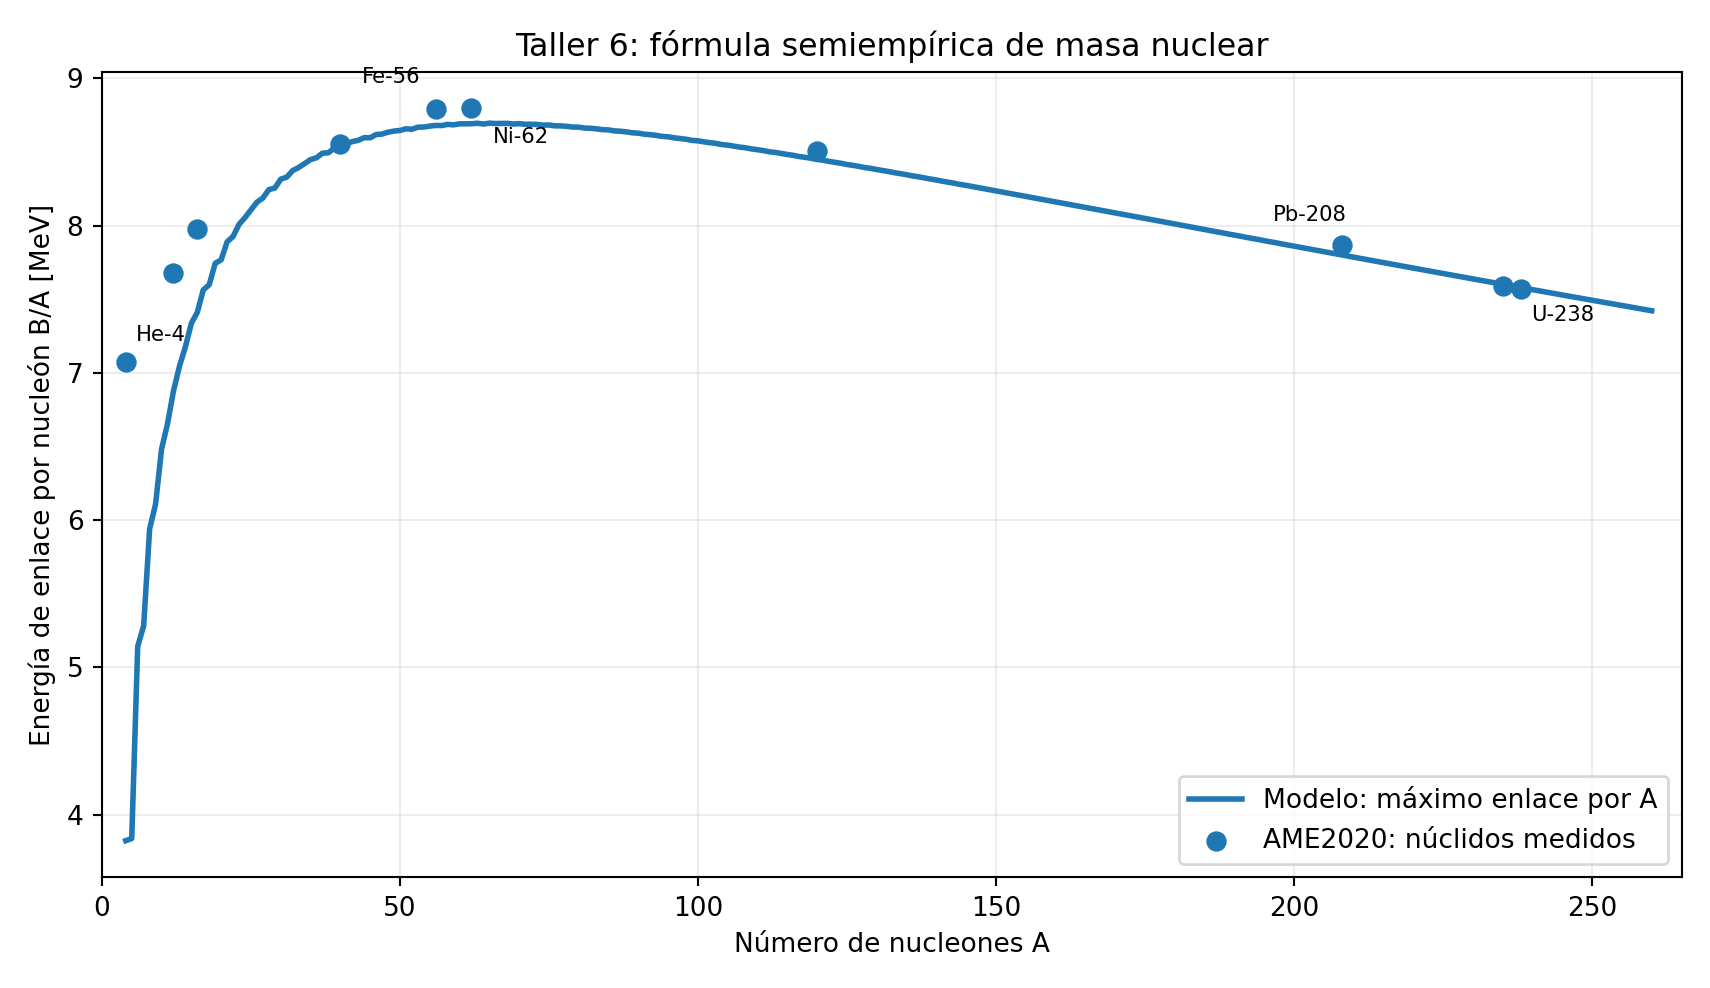
\includegraphics[width=0.75\textwidth]{taller_nucleo_atomico/curva_enlace.png}\\[-3pt]
{\footnotesize Figura 1. Curva de máximo enlace del modelo y diez núclidos experimentales.}
\end{center}
\vspace{-5pt}
\textbf{Verificación (PASS/FAIL):} 4 de 4 PASS con la celda original; 257 de 257 búsquedas de $Z$ correctas.

\textbf{4. Obstáculo o decisión de implementación.} Se evitó la división entera de Fortran en $A^{-1/3}$ y $A/2$ usando \texttt{real(a,dp)} y exponentes reales. También se compiló el módulo antes del programa y se declararon los argumentos con \texttt{intent(in/out)} para evitar modificaciones accidentales.

\textbf{5. Conclusión.} Para $A=56$, el modelo base prefiere $Z=25$ sobre Fe ($Z=26$) por $1.18775$ MeV de energía total. Al añadir \emph{solo para comparar} el apareamiento, Fe pasa a ser más ligado por $2.01939$ MeV; el resultado evidencia una limitación del modelo de cuatro términos.

\textbf{6. Uso de herramientas de IA.} Se utilizó ChatGPT para desarrollar y depurar código, organizar los módulos, apoyar la interpretación y preparar un borrador de este informe; los valores se contrastaron con las cuatro verificaciones del notebook del curso.

\vspace{2pt}\hrule\vspace{3pt}
{\footnotesize Código y resultados: \texttt{Taller\_6/taller\_nucleo\_atomico/}. Notebook ejecutado en \texttt{Taller\_6/}.}
\end{document}
